\documentclass[a4paper,oneside,11pt]{article}
\usepackage{ctex}
\usepackage{graphicx}
\usepackage{geometry}
\geometry{left = 2.5cm, right = 2.5cm, top = 2cm, bottom = 2cm}

\newcommand{\bol}[1]{\textbf{#1}}
\newcommand{\diff}{\mathrm{d}}

\title{刘维烨专用资料}
\author{Xiaoyu Xue}
\date{\today}

\begin{document}
\maketitle
\section{数学}
\subsection{数学符号}
\begin{enumerate}
	\item 求和: $\displaystyle \sum_{i = 0} ^ n a_i = a_0 + \ldots + a_n$
	\item 坐标: 三维坐标用$(x,y,z)$表示
	\item 向量: $\vec{a}$或者$\bol{a}$,三维向量$\bol{a} = (x,y,z)$
	\item 有限元差分: 用$\Delta x$来表示两个物理量$x1,~x2$的变化量
\end{enumerate}
\subsection{向量}
\subsubsection{向量的长度}
$\bol{a} = (x_1, y_1, z_1)$,向量$\bol{a}$的长度为
\begin{displaymath}
\vert \bol{a} \vert = \sqrt{x_1^2 + y_1^2 + z_1^2}
\end{displaymath}
\subsubsection{向量加法}
$\bol{a} = (x_1, y_1, z_1)$,$\bol{b} = (x_2, y_2, z_2)$,三角形或者平行四边形准则
\begin{displaymath}
\bol{a} + \bol{b} = (x_1 + x_2, y_1 + y_2, z_1 + z_2)
\end{displaymath}
\vspace{-10mm}
\begin{figure}[!h]
\centering
\includegraphics[scale=0.4]{./figure/fig1.eps}
\end{figure}
\subsubsection{向量数乘}
一个数乘一个向量的结果是一个向量
\begin{displaymath}
c\bol{a} = c(x, y, z) = (cx, cy, cz)
\end{displaymath}
\subsubsection{向量点乘}
向量点乘的结果是一个标量:
\begin{displaymath}
\bol{a} \cdot \bol{b} = \vert \bol{a}\vert \vert\bol{b}\vert \cos\theta =x_1x_2 + y_1y_2 + z_1z_2
\end{displaymath}
\subsubsection{向量叉乘}
向量叉乘的结果是一个向量,长度为
\begin{displaymath}
\vert\bol{a}\times\bol{b}\vert = \vert\bol{a}\vert \vert\bol{b}\vert \sin\theta
\end{displaymath}
\par 向量为:
\begin{displaymath}
\bol{a}\times\bol{b} = \left\vert
\begin{array}{ccc}
\bol{i} & \bol{j} & \bol{k}\\
x_1 & y_1 & z_1\\
x_2 & y_2 & z_2
\end{array}
\right\vert = \left(y_1z_2 - y_2z_1 , x_2z_1 - x_1z_2 , x_1y_2  - x_2y_1\right)
\end{displaymath}
\par 向量的方向根据坐标系选择左右手法则(不满足交换律)
\begin{figure}[!h]
\centering
\includegraphics[scale=0.3]{./figure/fig2.eps}
\end{figure}
\newpage
\section{位移、速度和加速度}
\subsection{位移}
定义:由初位置到末位置的一段有向线段(向量),单位: $m$\\
假设点A的位置为$\bol{a} = (x_1, y_1, z_1)$,点B的位置为$\bol{b} = (x_2, y_2, z_2)$,A到B的位移为$\bol{x} = \bol{b} - \bol{a} = (x_2 - x_1 , y_2 - y_1, z_2 - z_1)$

\subsection{速度}
定义:一个物体的速度定义成在某个参考系下它的位置的变换率,是一个随时间变化的函数,可以用$\bol{v}(t)$表示,单位: $m/s$\\
\subsubsection{平均速度(Average velocity)}
\begin{displaymath}
	\bar{\bol{v}} = \frac{\Delta \bol{x}}{\Delta t}
\end{displaymath}
其中$\Delta \bol{x}$表示位移,$\Delta t$表示经历的时间
\subsubsection{瞬时速度(Instantaneous velocity)}
\begin{displaymath}
	\bol{v} = \lim_{\Delta t \to 0}\frac{\Delta \bol{x}}{\Delta t} = \frac{\diff\bol{x}}{\diff t}
\end{displaymath}
因此位移可以通过瞬时速度的积分求得
\begin{displaymath}
\bol{x} = \int\bol{v}\diff t
\end{displaymath}
\subsection{加速度}
定义:加速度为速度随时间的变化率(向量),是一个时间的函数,用$\bol{a}(t)$表示,单位~$m/s^2$
\subsubsection{平均加速度(Average acceleration)}
\begin{displaymath}
	\bar{\bol{a}} = \frac{\Delta \bol{v}}{\Delta t}
\end{displaymath}
其中$\Delta \bol{v}$为速度差,$\Delta t$为经历的时间
\subsubsection{瞬时加速度(Instantaneous acceleration)}
\begin{displaymath}
	\bol{a} = \lim_{\Delta t \to 0} \frac{\Delta \bol{v}}{\Delta t} = \frac{\diff \bol{v}}{\diff t}
\end{displaymath}
可以看出瞬时加速度是速度随时间的导数,速度优势位移随时间的导数,所以加速度是位移随时间的二阶导数
\begin{displaymath}
	\bol{a} = \frac{\diff \bol{v}}{\diff t} = \frac{\diff^2 \bol{x}}{\diff t^2}
\end{displaymath}
\newpage
\section{受力分析}
\subsection{力}
在物理学中,力是任何导致自由物体历经速度、方向或外型的变化的影响。初中时候说过力的三要素:大小,方向和作用点。从这里就可以看出力是一个向量,力的字母表示通常是$\bol{F}$,经典力学通常涉及到牛顿运动定律,我们讨论的也都是经典力学的范围。力的单位为: 牛顿(N)
\begin{figure}[!h]
\centering
\includegraphics[scale=0.25]{./figure/fig3.eps}
\end{figure}
\subsection{力的种类}
\subsubsection{重力}
现在所称的重力,直到艾萨克·牛顿的工作之前,都没有被认定是万有的。这个朝向地球表面的由重力产生的加速度通常以 $\bol{g}$标示,有一个大约是9.81米每平方秒的大小(这个是从海平面测量且跟位置有关)且指向地心。 这个观测意味着地球表面上作用在物体上的重力直接地与物体质量成正比。因此一个有质量为$m$的物体所受的重力为
\begin{displaymath}
	\bol{G} = m\bol{g}
\end{displaymath}
\subsubsection{压力}
定义: 物理学上的压力,是指发生在两个物体的接触表面的作用力,或者是气体对于固体和液体表面的垂直作用力,或者是液体对于固体表面的垂直作用力。
\subsubsection{摩擦力}
定义: 摩擦力指两个表面接触的物体相对滑动时抵制它们的相对移动的力,是经典力学的一个名词。摩擦力又可以分为: 静摩擦,滑动摩擦和滚动摩擦。
\par 滑动摩擦力的大小可以用如下公式计算
\begin{displaymath}
F = \mu F_N
\end{displaymath}
其中$\mu$为摩擦系数,$F_N$为接触面的压力大小。
\subsubsection{弹力}
定义: 弹力是指发生弹性形变的物体由于要恢复原状,对他接触的物体产生的力。
\par 弹力大小用胡克定律计算: 弹簧发生弹性形变时,弹力的大小F跟弹簧伸长(或缩短)的长度x成正比
\begin{displaymath}
	F = -kx
\end{displaymath}
其中$k$是弹簧劲度系数,单位为$N/m$
\section{牛顿运动定律}
\subsection{牛顿第一定律}
牛顿第一定律表明,存在某些参考系,在其中,不受外力的物体都保持静止或匀速直线运动。
\begin{displaymath}
	\sum_i \bol{F}_i = 0 \Rightarrow \frac{\diff\bol{v}}{\diff t}
\end{displaymath}
其中$\bol{F}_i$是第$i$个外力,$\bol{v}$是速度,$t$是时间。
\subsection{牛顿第二定律}
牛顿第二定律表明,物体的加速度与施加的合外力成正比,与物体的质量成反比,方向与合外力方向相同。这定律又称为``加速度定律''。数学上,牛顿第二定律通常表达为:
\begin{displaymath}
	\bol{F} = m \bol{a}
\end{displaymath}
其中$m$为物体的质量,$\bol{a}$为加速度,从这里可以看出$1N = 1kg\cdot m/s^2$
\subsection{牛顿第三定律}
牛顿第三定律表明,当两个物体互相作用时,彼此施加于对方的力,其大小相等、方向相反:
\begin{displaymath}
	\sum \bol{F}_{AB} = \sum \bol{F}_{BA}
\end{displaymath}
其中$\bol{F}_{AB}$是物体B施加于物体A的力,$\bol{F}_{BA}$是物体A施加于物体B的力。
\newpage
\section{圆周运动}
\section{Try your best !}
\begin{figure}[!h]
\centering
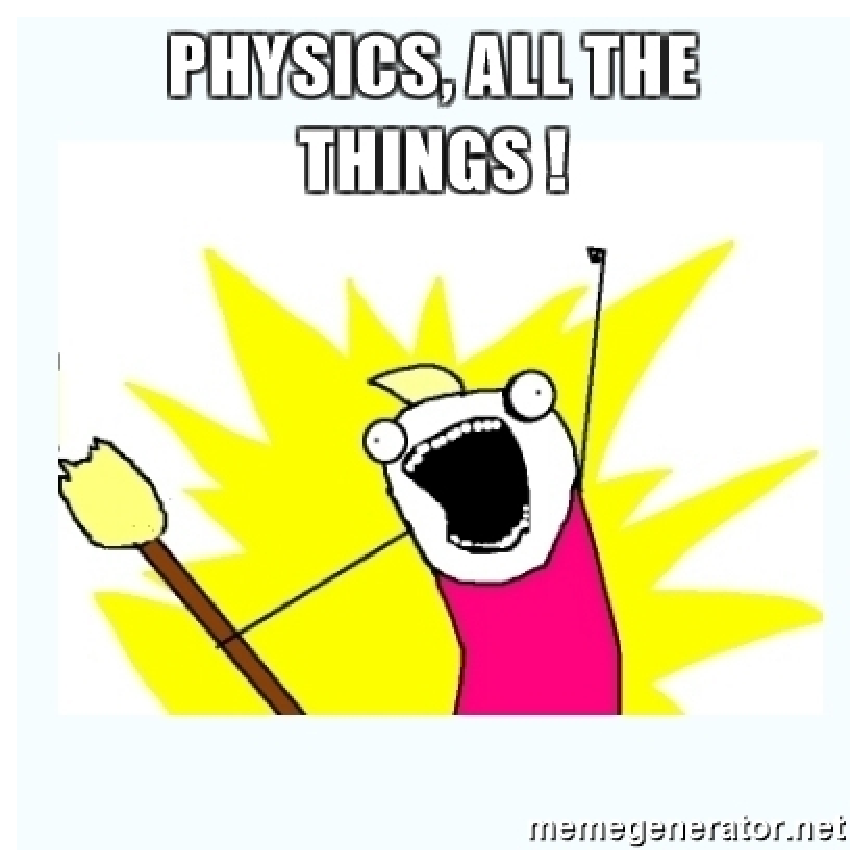
\includegraphics[scale=0.6]{./figure/fig0.eps}
\end{figure}
\end{document}